\documentclass[10pt]{extarticle}
\title{}
\author{}
\date{}
\usepackage[shortlabels]{enumitem}


%paper setup
\usepackage{geometry}
\geometry{letterpaper, portrait, margin=1in}
\usepackage{fancyhdr}
% sans serif font:
\usepackage{cmbright}
%symbols
\usepackage{amsmath}
\usepackage{bigints}
\usepackage{amssymb}
\usepackage{amsthm}
\usepackage{mathtools}
\usepackage[hidelinks]{hyperref}
\usepackage{gensymb}
\usepackage{multirow,array}
\usepackage{multicol}

\newtheorem*{remark}{Remark}
\usepackage[T1]{fontenc}
\usepackage[utf8]{inputenc}

%chemistry stuff
%\usepackage[version=4]{mhchem}
%\usepackage{chemfig}

%plotting
\usepackage{pgfplots}
\usepackage{tikz}
\tikzset{middleweight/.style={pos = 0.5}}
%\tikzset{weight/.style={pos = 0.5, fill = white}}
%\tikzset{lateweight/.style={pos = 0.75, fill = white}}
%\tikzset{earlyweight/.style={pos = 0.25, fill=white}}

%\usepackage{natbib}

%graphics stuff
\usepackage{graphicx}
\graphicspath{ {./images/} }
\usepackage[style=numeric, backend=biber]{biblatex} % Use the numeric style for Vancouver
\addbibresource{the_bibliography.bib}
%code stuff
%when using minted, make sure to add the -shell-escape flag
%you can use lstlisting if you don't want to use minted
%\usepackage{minted}
%\usemintedstyle{pastie}
%\newminted[javacode]{java}{frame=lines,framesep=2mm,linenos=true,fontsize=\footnotesize,tabsize=3,autogobble,}
%\newminted[cppcode]{cpp}{frame=lines,framesep=2mm,linenos=true,fontsize=\footnotesize,tabsize=3,autogobble,}

%\usepackage{listings}
%\usepackage{color}
%\definecolor{dkgreen}{rgb}{0,0.6,0}
%\definecolor{gray}{rgb}{0.5,0.5,0.5}
%\definecolor{mauve}{rgb}{0.58,0,0.82}
%
%\lstset{frame=tb,
%	language=Java,
%	aboveskip=3mm,
%	belowskip=3mm,
%	showstringspaces=false,
%	columns=flexible,
%	basicstyle={\small\ttfamily},
%	numbers=none,
%	numberstyle=\tiny\color{gray},
%	keywordstyle=\color{blue},
%	commentstyle=\color{dkgreen},
%	stringstyle=\color{mauve},
%	breaklines=true,
%	breakatwhitespace=true,
%	tabsize=3
%}
% text + color boxes
\renewcommand{\mathbf}[1]{\mathbold{#1}}
\usepackage[most]{tcolorbox}
\tcbuselibrary{breakable}
\tcbuselibrary{skins}
\newtcolorbox{problem}[1]{colback=white,enhanced,title={\small #1},
          attach boxed title to top center=
{yshift=-\tcboxedtitleheight/2},
boxed title style={size=small,colback=black!60!white}, sharp corners, breakable}
%including PDFs
%\usepackage{pdfpages}
\setlength{\parindent}{0pt}
\usepackage{cancel}
\pagestyle{fancy}
\fancyhf{}
\rhead{Avinash Iyer}
\lhead{Econ 308: Problem Set 9}
\newcommand{\card}{\text{card}}
\newcommand{\ran}{\text{ran}}
\newcommand{\N}{\mathbb{N}}
\newcommand{\Q}{\mathbb{Q}}
\newcommand{\Z}{\mathbb{Z}}
\newcommand{\R}{\mathbb{R}}
\begin{document}
  \begin{problem}{UBI vs. Workfare}
    This problem is a continuation of the in-class activity on Optimal Labor Income Taxes. Recall that all individuals have the same utility function over consumption and labor given by:
    \begin{align*}
      u(c,l) &= c-\frac{l^2}{2}
    \end{align*}
    where $c$ represents weekly consumption spending and $l$ represents hours of labor per week. Everyone earns an hourly wage $w$ that is taxed at rate $\tau$. In addition, each individual receives a weekly cash transfer $R$ from the government. The utility-maximizing labor supply choice is consequently $l^{\ast} = (1-\tau)w$.\\

    Now suppose that there are two individuals in the economy: low-wage Laura who earns \$20/hour, and high-wage Hanna who earns \$100/hour.
    \begin{problem}{(a)}
      Suppose the government implements the revenue-maximizing tax rate $\tau^{\ast} = 0.5$ and rebates total revenues equally back to Laura and Hanna. For both Laura and Hanna, determine their labor supply and consumption in this case.
      \tcblower
      \begin{description}[font=\normalfont]
        \item[Laura's Labor Supply:]
          \begin{align*}
            l^{\ast}_{L} &= (1-\tau)w\\
                     &= 10\text{ hours/week}\\
            R_1 &= (20)(0.5)(10)\\
                &= 100
          \end{align*}
        \item[Hanna's Labor Supply:]
          \begin{align*}
            l^{\ast}_{L} &= (1-\tau)(w)\\
                         &= 50\text{ hours/week}\\
            R_2 &= (100)(0.5)(50)\\
                &= 2500
          \end{align*}
        \item[Consumption:]
          \begin{align*}
            c_{L} &= (20)(0.5)(10) + 1300\\
                  &= 1400\\
            c_{H} &= (100)(0.5)(50) + 1300\\
                  &= 3800
          \end{align*}
      \end{description}
    \end{problem}
    \begin{problem}{(b)}
      Suppose there is an election and the new government administration abandons universal basic income, and changes the tax schedule such that
      \begin{itemize}
        \item There is a 100\% subsidy on the first \$1000 of weekly labor income.
        \item All weekly labor income above \$1000 is taxed at a rate of 50\%.
      \end{itemize}
      The new budget constraint in $(z,c)$ space is given below:
      \begin{center}
        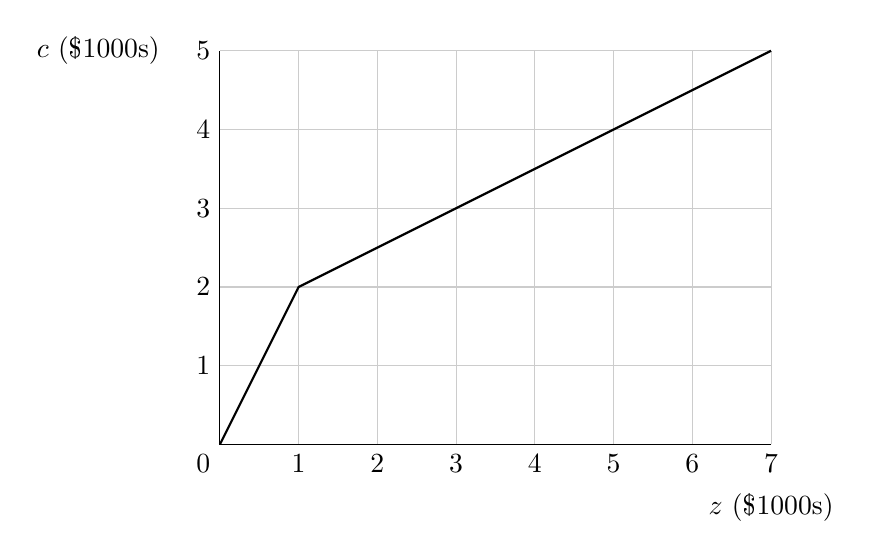
\begin{tikzpicture}
          \draw[black!20!white,thin](0,0) grid (7,5);
          \draw[thin] (7,0) -- (0,0) -- (0,5);
          \draw[thick] (0,0) -- (1,2) -- (7,5);
          \node[anchor = north] at (7,-0.5) {$z$ (\$1000s)};
          \node[anchor = north] at (1,0){$1$};
          \node[anchor = north] at (2,0){$2$};
          \node[anchor = north] at (3,0){$3$};
          \node[anchor = north] at (4,0){$4$};
          \node[anchor = north] at (5,0){$5$};
          \node[anchor = north] at (6,0){$6$};
          \node[anchor = north] at (7,0){$7$};
          \node[anchor = east] at (0,1){$1$};
          \node[anchor = east] at (0,2){$2$};
          \node[anchor = east] at (0,3){$3$};
          \node[anchor = east] at (0,4){$4$};
          \node[anchor = east] at (0,5){$5$};
          \node[anchor = north east] at (0,0){$0$};
          \node[anchor=east,text width=2.2cm] at (0,5) {$c$ (\$1000s)};
        \end{tikzpicture}
      \end{center}
      Find each individual's new labor supply and consumption.
      \tcblower
      \begin{description}[font=\normalfont]
        \item[Laura's Labor Supply and Consumption:]
          \begin{align*}
            l^{\ast}_{L} &= (1-\tau)w\\
                     &= 40\text{ hours/week}\\
            c_{L} &= (40)(40)\\
                     &= 1600
          \end{align*}
        \item[Hanna's Labor Supply and Consumption:]
          \begin{align*}
            l^{\ast}_{H} &= (1-\tau)w\\
                         &= 50\text{ hours/week}\\
              c &= (30)(50) + 1000\\
              &= 2500
          \end{align*}
      \end{description}
    \end{problem}
    \begin{problem}{(c)}
      Discuss the magnitude and sign of the substitution and income effects for Laura and Hanna's labor supply choices from this new tax policy relative to the previous tax scheme.
      \tcblower
      While the income effects for both Laura and Hanna were both negative in each scenario, the substitution effect was $0$ in the UBI scheme and positive in the second scheme for Laura, while it was $0$ and negative respectively for Hanna.
    \end{problem}
    \begin{problem}{(d)}
      Are Laura and Hanna each better off with the tax scheme from part (a) or part (b)? Is utilitarian social welfare higher under the tax scheme from part (a) or part (b)? Does your answer change with a Rawlsian social welfare function?
      \tcblower
      Laura is better off in the second tax scheme, while Hanna is worse off, relative to the first tax scheme. Utilitarian social welfare is reduced under the second scheme compared to the first scheme, while Rawlsian social welfare is increased.
    \end{problem}
  \end{problem}
  \begin{problem}{Trying UBI}
    A wealthy tech mogul, concerned about how increasing automation might one day reduce the ability of employment in some sectors of the economy, has decided to fund a randomized controlled trial of Universal Basic Income. The trial will last three years, and study 1,000 people randomly assigned to receive \$5,000 per year with no strings attached. Five hundred people will be randomly assigned to receive \$5,000 per year with no strings attached, and the other five hundred will receive only a small incentive to participate in the study. What are the advantages and pitfalls of such a research strategy in understanding the likely benefits and drawbacks of a Universal Basic Income implemented nationwide for all citizens?
    \tcblower
    The main advantage of a RCT is that it can provide much stronger proof of causality than quasi-experimental methods such as regression discontinuities or DD estimators. However, the problem of external validity remains --- there could be selection bias in who entered the RCT, and the results from the RCT may not be applicable to the general population.
  \end{problem}
  \begin{problem}{A Kinky Bunch}
    Consider an Earned Income Tax Credit (EITC) with the following structure:
    \begin{itemize}
      \item Phase-In: 50\% subsidy on the first \$10,000 of pre-tax earnings
      \item Plateau: 0\% marginal tax rate on pre-tax earnings between \$10,000 and \$20,000
      \item Phase-Out: Pre-tax earnings above \$20,000 are taxed at a 25\% rate until the credit is fully phased out.
    \end{itemize}
    \begin{problem}{(a)}
      \begin{center}
        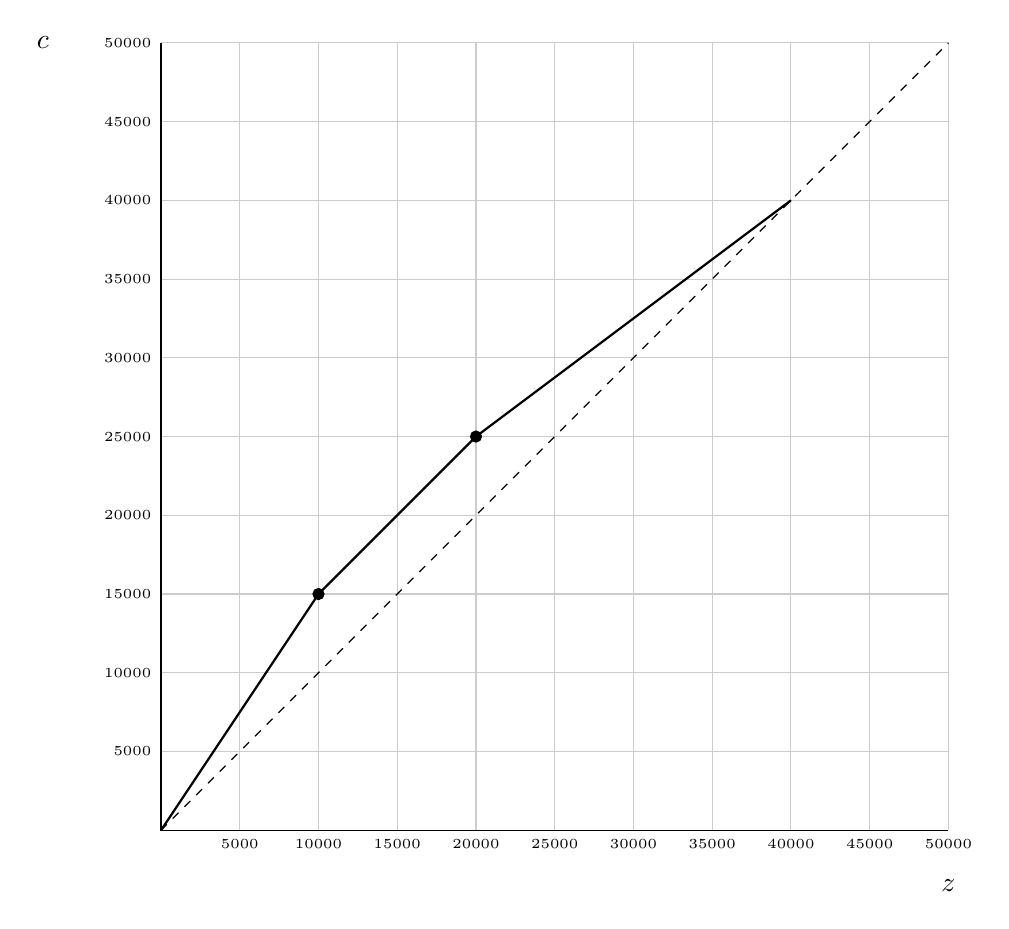
\begin{tikzpicture}
          \draw[black!20!white,thin] (0,0) grid (10,10);
          \draw (10,0) -- (0,0) -- (0,10);
          \node[anchor = east] at (0,1){\tiny $5000$};
          \node[anchor = east] at (0,2){\tiny $10000$};
          \node[anchor = east] at (0,3){\tiny $15000$};
          \node[anchor = east] at (0,4){\tiny $20000$};
          \node[anchor = east] at (0,5){\tiny $25000$};
          \node[anchor = east] at (0,6){\tiny $30000$};
          \node[anchor = east] at (0,7){\tiny $35000$};
          \node[anchor = east] at (0,8){\tiny $40000$};
          \node[anchor = east] at (0,9){\tiny $45000$};
          \node[anchor = east] at (0,10){\tiny $50000$};

          \node[anchor = north] at (1,0){\tiny $5000$};
          \node[anchor = north] at (2,0){\tiny $10000$};
          \node[anchor = north] at (3,0){\tiny $15000$};
          \node[anchor = north] at (4,0){\tiny $20000$};
          \node[anchor = north] at (5,0){\tiny $25000$};
          \node[anchor = north] at (6,0){\tiny $30000$};
          \node[anchor = north] at (7,0){\tiny $35000$};
          \node[anchor = north] at (8,0){\tiny $40000$};
          \node[anchor = north] at (9,0){\tiny $45000$};
          \node[anchor = north] at (10,0){\tiny $50000$};

          \node[anchor = north] at (10,-0.5) {$z$};
          \node[anchor = east] at (-1.3,10) {$c$};
          \draw[thick] (0,0) -- (2,3) -- (4,5) -- (8,8);
          \draw[dashed] (0,0) -- (10,10);
          \filldraw (2,3) circle (2pt)
                    (4,5) circle (2pt);
        \end{tikzpicture}
      \end{center}
    \end{problem}
    Each individual supplies the following hours per year:
    \begin{align*}
      l^{\ast} &= \left(w(1-\tau)\right)^3
    \end{align*}
    where $w$ is the market hourly wage and $\tau$ is the marginal tax rate on earnings. Observe that there are no labor supply income effects.
    \begin{problem}{(b)}
      What is an individual's annual market earnings $z$ as a function of $\tau$ and $w$?
      \tcblower
      \begin{align*}
        z &= wl^{\ast}\\
          &= w^{4}(1-\tau)^{3}
      \end{align*}
    \end{problem}
    The following three individuals differ only in their wages:
    \begin{itemize}
      \item Low-wage Lola makes \$8/hour
      \item Medium-wage Maria makes \$11/hour
      \item High-wage Harper makes \$13/hour
    \end{itemize}
    \begin{problem}{(c)}
      For each individual, determine their choice of $z$ with and without the EITC.
      \tcblower
      \begin{description}[font=\normalfont]
        \item[Lola without EITC:]
          \begin{align*}
            z &= (8)^4\\
                     &= 4096
          \end{align*}
        \item[Lola with EITC:]
          \begin{align*}
            z' &= w^{4}(1-\tau)^{3}\\
               &= 13824 \tag*{within $50\%$ subsidy, so valid}
          \end{align*}
        \item[Maria without EITC:]
          \begin{align*}
            z &= (11)^{4}\\
              &= 14641
          \end{align*}
        \item[Maria with EITC:]
          \begin{align*}
            z' &= 5000 + (11)^{4}\\
               &= 19641 \tag*{within $0\%$ subsidy, so valid}
          \end{align*}
        \item[Harper without EITC:]
          \begin{align*}
            z &= (13)^{4}\\
              &= 28561
          \end{align*}
        \item[Harper with EITC:]
          \begin{align*}
            z'_{1} &= (1-0.25)^3(13^4)\tag*{assume in $25\%$ tax}\\
              &= \xcancel{12049} \tag*{not within $25\%$ tax}\\
            z'_{2} &= 13^{4} + 5000 \tag*{assume within $0\%$ tax}\\
                   &= \xcancel{33561}\\
            z' &= 25000 \tag*{must be that Harper bunches at kink}
          \end{align*}
      \end{description}
    \end{problem}
    \begin{problem}{(d)}
      Briefly explain why the theoretical predictions of EITC in part (c) may deviate from empirical evidence.
      \tcblower
      There may not be bunching (as was the case with Harper) if certain aspects such as employment contracts are fixed for a period of time (i.e., substitution effect is muted). Alternatively, the income effects may be stronger than zero, making the effect of the EITC to decrease work hours further than was expected.
    \end{problem}
  \end{problem}
  \begin{problem}{Danish Differences}
    Kleven and Schultz (2014) estimate the elasticity of taxable income using the full population of tax revenues in Denmark since 1980. In particular, Denmark changed its marginal tax rates as part of a 1987 tax reform, lowering (increasing) tax rates on high (low) labor and capital income.
    \begin{problem}{(a)}
      Provide a brief interpretation of the visual evidence. In particular, what qualitatively do the figures show about the impact of tax rates on both labor and capital income?
      \tcblower
      We see from the graphs that upon implementation, incomes in both capital and labor increase in the case where there are tax cuts relative to ones where there are tax increases.
    \end{problem}
    \begin{problem}{(b)}
      In each figure they also report the DD estimate of the taxable income elasticity. What assumption must hold for the DD estimator to identify the causal effect of the tax changes? Does it appear that this assumption holds?
      \tcblower
      The assumption that must hold for the DD estimator to hold is the parallel trends --- i.e., the track of capital/labor income would have been the same in absence of the tax change. It does appear to be the case, seeing as lower capital and labor income tracked their higher counterparts before the tax change.
    \end{problem}
    \begin{problem}{(c)}
      Is the taxable income elasticity larger for labor or capital income?
      \tcblower
      The taxable income elasticity is higher for capital income than for labor income; this is likely because it is easier to ``pull back'' from higher-taxed capital (by consuming more), while it is harder to ``pull back'' from higher-taxed labor due to the existence of stronger employment contracts.
    \end{problem}
  \end{problem}
\end{document}
